\batchmode
\documentclass[twoside]{book}

% Packages required by doxygen
\usepackage{fixltx2e}
\usepackage{calc}
\usepackage{doxygen}
\usepackage[export]{adjustbox} % also loads graphicx
\usepackage{graphicx}
\usepackage[utf8]{inputenc}
\usepackage{makeidx}
\usepackage{multicol}
\usepackage{multirow}
\PassOptionsToPackage{warn}{textcomp}
\usepackage{textcomp}
\usepackage[nointegrals]{wasysym}
\usepackage[table]{xcolor}

% Font selection
\usepackage[T1]{fontenc}
\usepackage[scaled=.90]{helvet}
\usepackage{courier}
\usepackage{amssymb}
\usepackage{sectsty}
\renewcommand{\familydefault}{\sfdefault}
\allsectionsfont{%
  \fontseries{bc}\selectfont%
  \color{darkgray}%
}
\renewcommand{\DoxyLabelFont}{%
  \fontseries{bc}\selectfont%
  \color{darkgray}%
}
\newcommand{\+}{\discretionary{\mbox{\scriptsize$\hookleftarrow$}}{}{}}

% Page & text layout
\usepackage{geometry}
\geometry{%
  a4paper,%
  top=2.5cm,%
  bottom=2.5cm,%
  left=2.5cm,%
  right=2.5cm%
}
\tolerance=750
\hfuzz=15pt
\hbadness=750
\setlength{\emergencystretch}{15pt}
\setlength{\parindent}{0cm}
\setlength{\parskip}{3ex plus 2ex minus 2ex}
\makeatletter
\renewcommand{\paragraph}{%
  \@startsection{paragraph}{4}{0ex}{-1.0ex}{1.0ex}{%
    \normalfont\normalsize\bfseries\SS@parafont%
  }%
}
\renewcommand{\subparagraph}{%
  \@startsection{subparagraph}{5}{0ex}{-1.0ex}{1.0ex}{%
    \normalfont\normalsize\bfseries\SS@subparafont%
  }%
}
\makeatother

% Headers & footers
\usepackage{fancyhdr}
\pagestyle{fancyplain}
\fancyhead[LE]{\fancyplain{}{\bfseries\thepage}}
\fancyhead[CE]{\fancyplain{}{}}
\fancyhead[RE]{\fancyplain{}{\bfseries\leftmark}}
\fancyhead[LO]{\fancyplain{}{\bfseries\rightmark}}
\fancyhead[CO]{\fancyplain{}{}}
\fancyhead[RO]{\fancyplain{}{\bfseries\thepage}}
\fancyfoot[LE]{\fancyplain{}{}}
\fancyfoot[CE]{\fancyplain{}{}}
\fancyfoot[RE]{\fancyplain{}{\bfseries\scriptsize Generated by Doxygen }}
\fancyfoot[LO]{\fancyplain{}{\bfseries\scriptsize Generated by Doxygen }}
\fancyfoot[CO]{\fancyplain{}{}}
\fancyfoot[RO]{\fancyplain{}{}}
\renewcommand{\footrulewidth}{0.4pt}
\renewcommand{\chaptermark}[1]{%
  \markboth{#1}{}%
}
\renewcommand{\sectionmark}[1]{%
  \markright{\thesection\ #1}%
}

% Indices & bibliography
\usepackage{natbib}
\usepackage[titles]{tocloft}
\setcounter{tocdepth}{3}
\setcounter{secnumdepth}{5}
\makeindex

% Hyperlinks (required, but should be loaded last)
\usepackage{ifpdf}
\ifpdf
  \usepackage[pdftex,pagebackref=true]{hyperref}
\else
  \usepackage[ps2pdf,pagebackref=true]{hyperref}
\fi
\hypersetup{%
  colorlinks=true,%
  linkcolor=blue,%
  citecolor=blue,%
  unicode%
}

% Custom commands
\newcommand{\clearemptydoublepage}{%
  \newpage{\pagestyle{empty}\cleardoublepage}%
}

\usepackage{caption}
\captionsetup{labelsep=space,justification=centering,font={bf},singlelinecheck=off,skip=4pt,position=top}

%===== C O N T E N T S =====

\begin{document}

% Titlepage & ToC
\hypersetup{pageanchor=false,
             bookmarksnumbered=true
            }
\pagenumbering{alph}
\pagenumbering{arabic}
\hypersetup{pageanchor=true}

%--- Begin generated contents ---
\chapter{Thermoelasticity\+: Combining the Heat equation and non-\/linear Solid Mechanics}
\label{index}\hypertarget{index}{}\hypertarget{index_q}{}\section{A few quick questions...}\label{index_q}
Since {\ttfamily oomph-\/lib} is developed as open-\/source software, any evidence that the code is being downloaded and used is very helpful for us as it helps to justify our continued work on this project.

We would therefore be extremely grateful if you could provide the information requested in the form below. Pressing the \char`\"{}submit\char`\"{} button will get you to the actual download page.

{\bfseries Note\+:} 
\begin{DoxyItemize}
\item All information will be treated as confidential. 
\item If you provide your email address and check the appropriate box we will add you to our mailing list to inform you of upgrades and bug fixes to the code. Rest assured that the mailing list is {\bfseries very low volume} -- we have better things to do than to bombard you with email. 
\item If you still feel reluctant to provide any of the information requested, feel free to enter some dummy input. The form will check that {\bfseries some} information has been entered but entering your name as \char`\"{}\+Joe Cool\char`\"{} is perfectly acceptable -- this is to discourage people from not providing the information simply because they are too lazy to type... 
\end{DoxyItemize}



 







 

 \hypertarget{index_pdf}{}\section{P\+D\+F file}\label{index_pdf}
A \href{../latex/refman.pdf}{\tt pdf version} of this document is available. \end{document}

\chapter{Namespace Index}
\section{Namespace List}
Here is a list of all namespaces with brief descriptions\+:\begin{DoxyCompactList}
\item\contentsline{section}{\hyperlink{namespaceGlobal__Physical__Variables}{Global\+\_\+\+Physical\+\_\+\+Variables} \\*Global variables that represent physical properties }{\pageref{namespaceGlobal__Physical__Variables}}{}
\item\contentsline{section}{\hyperlink{namespaceoomph}{oomph} }{\pageref{namespaceoomph}}{}
\item\contentsline{section}{\hyperlink{namespacePhysical__Variables}{Physical\+\_\+\+Variables} \\*Namespace for the solution of 2D linear shell equation }{\pageref{namespacePhysical__Variables}}{}
\end{DoxyCompactList}

\chapter{Hierarchical Index}
\section{Class Hierarchy}
This inheritance list is sorted roughly, but not completely, alphabetically\+:\begin{DoxyCompactList}
\item Problem\begin{DoxyCompactList}
\item \contentsline{section}{Unstructured\+Solid\+Problem$<$ E\+L\+E\+M\+E\+NT $>$}{\pageref{classUnstructuredSolidProblem}}{}
\end{DoxyCompactList}
\end{DoxyCompactList}

\chapter{Class Index}
\section{Class List}
Here are the classes, structs, unions and interfaces with brief descriptions\+:\begin{DoxyCompactList}
\item\contentsline{section}{\hyperlink{classPMLProblem}{P\+M\+L\+Problem$<$ E\+L\+E\+M\+E\+N\+T $>$} }{\pageref{classPMLProblem}}{}
\item\contentsline{section}{\hyperlink{classGlobalParameters_1_1TestPMLMapping}{Global\+Parameters\+::\+Test\+P\+M\+L\+Mapping} }{\pageref{classGlobalParameters_1_1TestPMLMapping}}{}
\end{DoxyCompactList}

\chapter{File Index}
\section{File List}
Here is a list of all files with brief descriptions\+:\begin{DoxyCompactList}
\item\contentsline{section}{\hyperlink{jeffery__orbit_8cc}{jeffery\+\_\+orbit.\+cc} }{\pageref{jeffery__orbit_8cc}}{}
\item\contentsline{section}{\hyperlink{jeffery__orbit_8txt__doxygenified_8h}{jeffery\+\_\+orbit.\+txt\+\_\+doxygenified.\+h} }{\pageref{jeffery__orbit_8txt__doxygenified_8h}}{}
\item\contentsline{section}{\hyperlink{my__taylor__hood__elements_8h}{my\+\_\+taylor\+\_\+hood\+\_\+elements.\+h} }{\pageref{my__taylor__hood__elements_8h}}{}
\end{DoxyCompactList}

\chapter{Namespace Documentation}
\hypertarget{namespaceGlobal__Physical__Variables}{}\section{Global\+\_\+\+Physical\+\_\+\+Variables Namespace Reference}
\label{namespaceGlobal__Physical__Variables}\index{Global\+\_\+\+Physical\+\_\+\+Variables@{Global\+\_\+\+Physical\+\_\+\+Variables}}


Namespace for physical parameters.  


\subsection*{Functions}
\begin{DoxyCompactItemize}
\item 
Vector$<$ double $>$ \hyperlink{namespaceGlobal__Physical__Variables_afae321364975eb56688ad13abc8ed6b7}{Gravity} (2)
\begin{DoxyCompactList}\small\item\em Gravity vector. \end{DoxyCompactList}\item 
void \hyperlink{namespaceGlobal__Physical__Variables_a87da705b8a46bed337cf5dbdd788b87b}{body\+\_\+force} (const double \&time, const Vector$<$ double $>$ \&x, Vector$<$ double $>$ \&result)
\begin{DoxyCompactList}\small\item\em Functional body force. \end{DoxyCompactList}\item 
void \hyperlink{namespaceGlobal__Physical__Variables_a9780d615ae07c4e00a436ab2973b54e6}{zero\+\_\+body\+\_\+force} (const double \&time, const Vector$<$ double $>$ \&x, Vector$<$ double $>$ \&result)
\begin{DoxyCompactList}\small\item\em Zero functional body force. \end{DoxyCompactList}\end{DoxyCompactItemize}
\subsection*{Variables}
\begin{DoxyCompactItemize}
\item 
double \hyperlink{namespaceGlobal__Physical__Variables_ab814e627d2eb5bc50318879d19ab16b9}{Re} =100
\begin{DoxyCompactList}\small\item\em Reynolds number. \end{DoxyCompactList}\item 
double \hyperlink{namespaceGlobal__Physical__Variables_ab1a845a672b4d74b304639a976dc65c6}{Re\+\_\+inv\+Fr} =100
\begin{DoxyCompactList}\small\item\em Reynolds/\+Froude number. \end{DoxyCompactList}\end{DoxyCompactItemize}


\subsection{Detailed Description}
Namespace for physical parameters. 

\subsection{Function Documentation}
\mbox{\Hypertarget{namespaceGlobal__Physical__Variables_a87da705b8a46bed337cf5dbdd788b87b}\label{namespaceGlobal__Physical__Variables_a87da705b8a46bed337cf5dbdd788b87b}} 
\index{Global\+\_\+\+Physical\+\_\+\+Variables@{Global\+\_\+\+Physical\+\_\+\+Variables}!body\+\_\+force@{body\+\_\+force}}
\index{body\+\_\+force@{body\+\_\+force}!Global\+\_\+\+Physical\+\_\+\+Variables@{Global\+\_\+\+Physical\+\_\+\+Variables}}
\subsubsection{\texorpdfstring{body\+\_\+force()}{body\_force()}}
{\footnotesize\ttfamily void Global\+\_\+\+Physical\+\_\+\+Variables\+::body\+\_\+force (\begin{DoxyParamCaption}\item[{const double \&}]{time,  }\item[{const Vector$<$ double $>$ \&}]{x,  }\item[{Vector$<$ double $>$ \&}]{result }\end{DoxyParamCaption})}



Functional body force. 



Definition at line 62 of file circular\+\_\+driven\+\_\+cavity.\+cc.



References Re\+\_\+inv\+Fr.



Referenced by main().

\mbox{\Hypertarget{namespaceGlobal__Physical__Variables_afae321364975eb56688ad13abc8ed6b7}\label{namespaceGlobal__Physical__Variables_afae321364975eb56688ad13abc8ed6b7}} 
\index{Global\+\_\+\+Physical\+\_\+\+Variables@{Global\+\_\+\+Physical\+\_\+\+Variables}!Gravity@{Gravity}}
\index{Gravity@{Gravity}!Global\+\_\+\+Physical\+\_\+\+Variables@{Global\+\_\+\+Physical\+\_\+\+Variables}}
\subsubsection{\texorpdfstring{Gravity()}{Gravity()}}
{\footnotesize\ttfamily Vector$<$double$>$ Global\+\_\+\+Physical\+\_\+\+Variables\+::\+Gravity (\begin{DoxyParamCaption}\item[{2}]{ }\end{DoxyParamCaption})}



Gravity vector. 



Referenced by main(), and Quarter\+Circle\+Driven\+Cavity\+Problem$<$ E\+L\+E\+M\+E\+N\+T $>$\+::\+Quarter\+Circle\+Driven\+Cavity\+Problem().

\mbox{\Hypertarget{namespaceGlobal__Physical__Variables_a9780d615ae07c4e00a436ab2973b54e6}\label{namespaceGlobal__Physical__Variables_a9780d615ae07c4e00a436ab2973b54e6}} 
\index{Global\+\_\+\+Physical\+\_\+\+Variables@{Global\+\_\+\+Physical\+\_\+\+Variables}!zero\+\_\+body\+\_\+force@{zero\+\_\+body\+\_\+force}}
\index{zero\+\_\+body\+\_\+force@{zero\+\_\+body\+\_\+force}!Global\+\_\+\+Physical\+\_\+\+Variables@{Global\+\_\+\+Physical\+\_\+\+Variables}}
\subsubsection{\texorpdfstring{zero\+\_\+body\+\_\+force()}{zero\_body\_force()}}
{\footnotesize\ttfamily void Global\+\_\+\+Physical\+\_\+\+Variables\+::zero\+\_\+body\+\_\+force (\begin{DoxyParamCaption}\item[{const double \&}]{time,  }\item[{const Vector$<$ double $>$ \&}]{x,  }\item[{Vector$<$ double $>$ \&}]{result }\end{DoxyParamCaption})}



Zero functional body force. 



Definition at line 70 of file circular\+\_\+driven\+\_\+cavity.\+cc.



Referenced by main().



\subsection{Variable Documentation}
\mbox{\Hypertarget{namespaceGlobal__Physical__Variables_ab814e627d2eb5bc50318879d19ab16b9}\label{namespaceGlobal__Physical__Variables_ab814e627d2eb5bc50318879d19ab16b9}} 
\index{Global\+\_\+\+Physical\+\_\+\+Variables@{Global\+\_\+\+Physical\+\_\+\+Variables}!Re@{Re}}
\index{Re@{Re}!Global\+\_\+\+Physical\+\_\+\+Variables@{Global\+\_\+\+Physical\+\_\+\+Variables}}
\subsubsection{\texorpdfstring{Re}{Re}}
{\footnotesize\ttfamily double Global\+\_\+\+Physical\+\_\+\+Variables\+::\+Re =100}



Reynolds number. 



Definition at line 53 of file circular\+\_\+driven\+\_\+cavity.\+cc.



Referenced by Quarter\+Circle\+Driven\+Cavity\+Problem$<$ E\+L\+E\+M\+E\+N\+T $>$\+::\+Quarter\+Circle\+Driven\+Cavity\+Problem().

\mbox{\Hypertarget{namespaceGlobal__Physical__Variables_ab1a845a672b4d74b304639a976dc65c6}\label{namespaceGlobal__Physical__Variables_ab1a845a672b4d74b304639a976dc65c6}} 
\index{Global\+\_\+\+Physical\+\_\+\+Variables@{Global\+\_\+\+Physical\+\_\+\+Variables}!Re\+\_\+inv\+Fr@{Re\+\_\+inv\+Fr}}
\index{Re\+\_\+inv\+Fr@{Re\+\_\+inv\+Fr}!Global\+\_\+\+Physical\+\_\+\+Variables@{Global\+\_\+\+Physical\+\_\+\+Variables}}
\subsubsection{\texorpdfstring{Re\+\_\+inv\+Fr}{Re\_invFr}}
{\footnotesize\ttfamily double Global\+\_\+\+Physical\+\_\+\+Variables\+::\+Re\+\_\+inv\+Fr =100}



Reynolds/\+Froude number. 



Definition at line 56 of file circular\+\_\+driven\+\_\+cavity.\+cc.



Referenced by body\+\_\+force(), and Quarter\+Circle\+Driven\+Cavity\+Problem$<$ E\+L\+E\+M\+E\+N\+T $>$\+::\+Quarter\+Circle\+Driven\+Cavity\+Problem().


\chapter{Class Documentation}
\hypertarget{classQThermalPVDElement}{}\section{Q\+Thermal\+P\+V\+D\+Element$<$ D\+IM $>$ Class Template Reference}
\label{classQThermalPVDElement}\index{Q\+Thermal\+P\+V\+D\+Element$<$ D\+I\+M $>$@{Q\+Thermal\+P\+V\+D\+Element$<$ D\+I\+M $>$}}
Inheritance diagram for Q\+Thermal\+P\+V\+D\+Element$<$ D\+IM $>$\+:\begin{figure}[H]
\begin{center}
\leavevmode
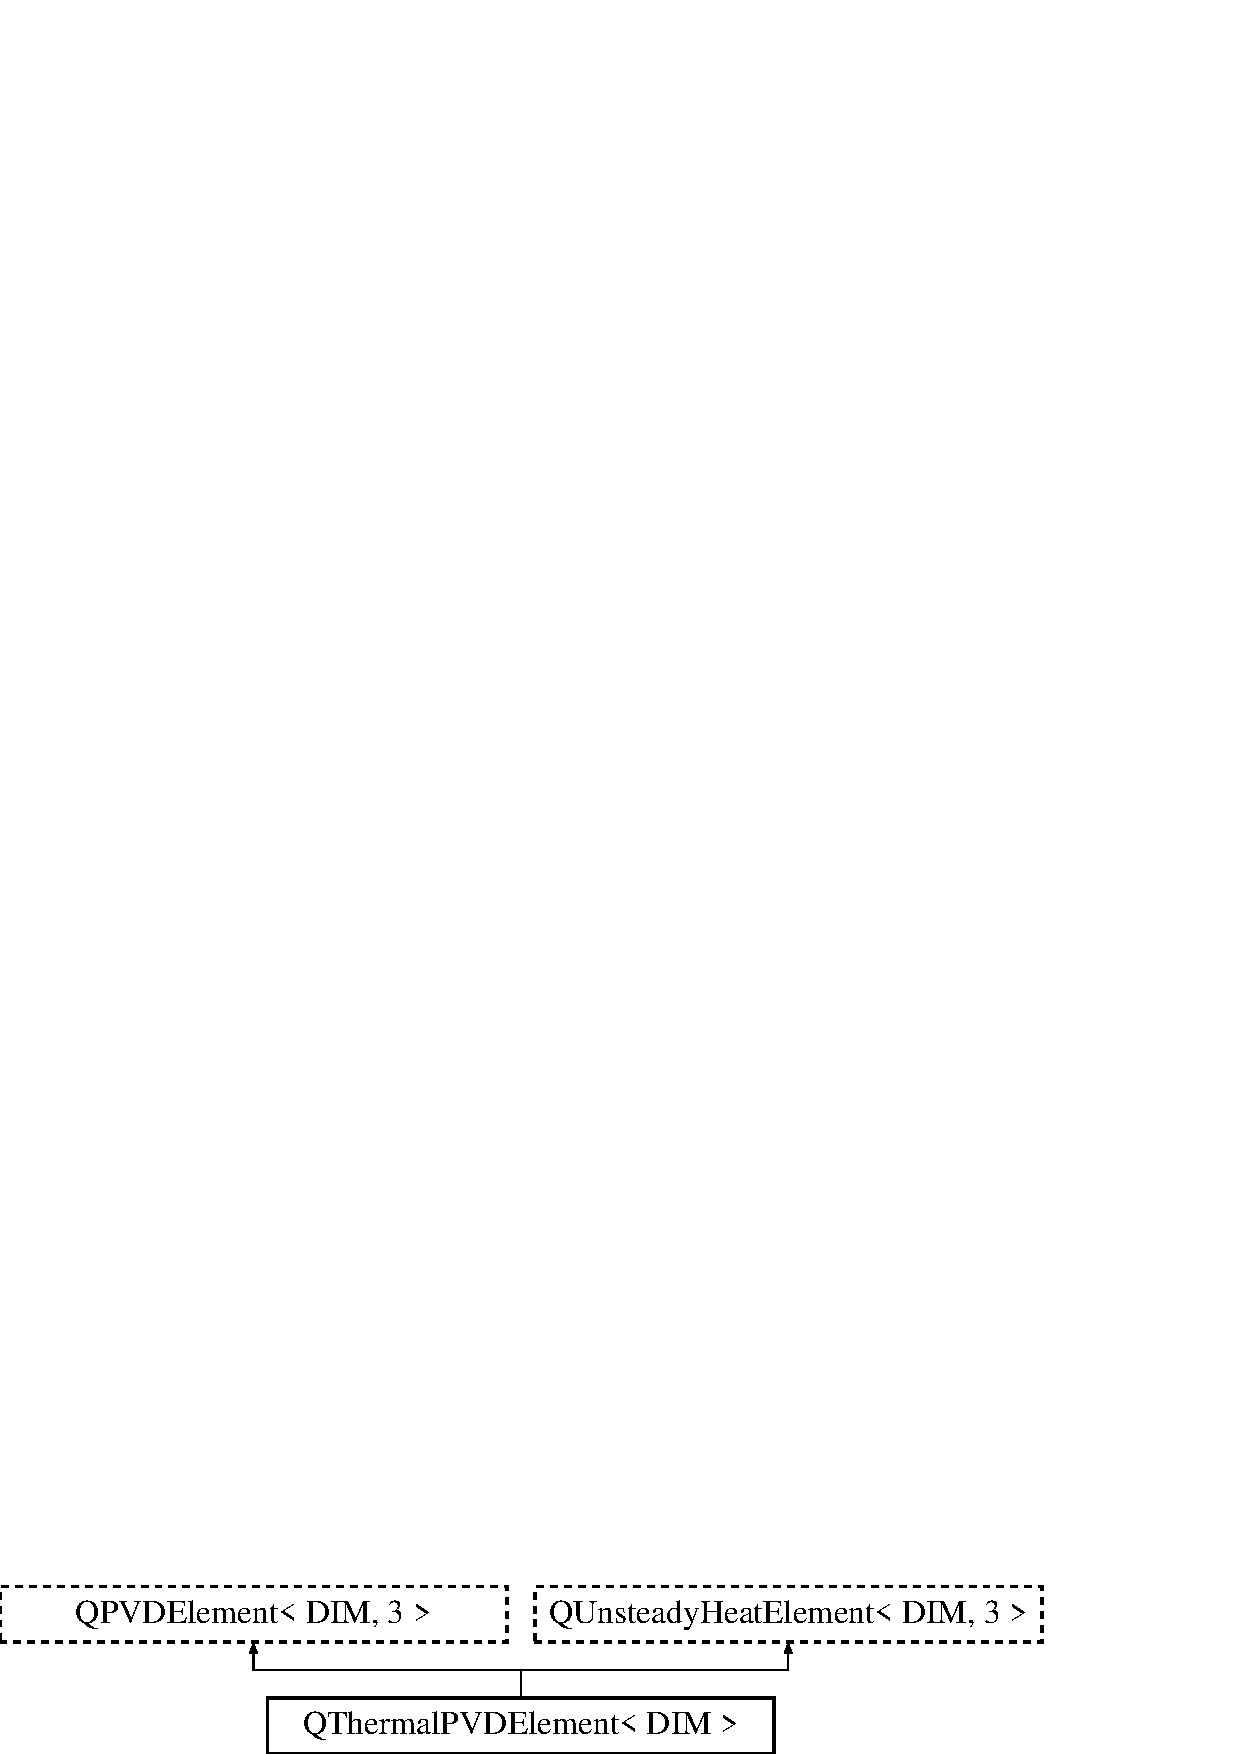
\includegraphics[height=2.000000cm]{classQThermalPVDElement}
\end{center}
\end{figure}
\subsection*{Public Member Functions}
\begin{DoxyCompactItemize}
\item 
\hyperlink{classQThermalPVDElement_a24d60d6461b169603388f263cbdccd75}{Q\+Thermal\+P\+V\+D\+Element} ()
\begin{DoxyCompactList}\small\item\em Constructor\+: call the underlying constructors and initialise the pointer to Alpha to point to the default value of 1.\+0. \end{DoxyCompactList}\item 
unsigned \hyperlink{classQThermalPVDElement_a55025994fc3d2799fde6f9c1142340af}{required\+\_\+nvalue} (const unsigned \&n) const
\begin{DoxyCompactList}\small\item\em The required number of values stored at the nodes is the sum of the required values of the two single-\/physics elements. Note that this step is generic for any multi-\/physics element of this type. \end{DoxyCompactList}\item 
const double \& \hyperlink{classQThermalPVDElement_a59b86e75dc7b6f99a84ef17fef8d949d}{alpha} () const
\begin{DoxyCompactList}\small\item\em Access function for the thermal expansion coefficient (const version) \end{DoxyCompactList}\item 
double $\ast$\& \hyperlink{classQThermalPVDElement_a57fb80dd582c02c0e8c7dc17491bf76f}{alpha\+\_\+pt} ()
\begin{DoxyCompactList}\small\item\em Access function for the pointer to the thermal expansion coefficientr. \end{DoxyCompactList}\item 
void \hyperlink{classQThermalPVDElement_a99e482f47a98c1b5ec7ec069211de827}{output} (ostream \&outfile)
\begin{DoxyCompactList}\small\item\em Overload the standard output function with the broken default. \end{DoxyCompactList}\item 
void \hyperlink{classQThermalPVDElement_a9d00cc21789124a37dffc9fdf2f011cd}{output} (ostream \&outfile, const unsigned \&nplot)
\begin{DoxyCompactList}\small\item\em Output function\+: Output x, y, u, v, p, theta at Nplot$^\wedge$\+D\+IM plot points. \end{DoxyCompactList}\item 
void \hyperlink{classQThermalPVDElement_af290922dfcefef30dc03fca2a2cb4fbf}{output} (F\+I\+LE $\ast$file\+\_\+pt)
\begin{DoxyCompactList}\small\item\em C-\/style output function\+: Broken default. \end{DoxyCompactList}\item 
void \hyperlink{classQThermalPVDElement_a649062cd4f15d8f14a2755786dd466dc}{output} (F\+I\+LE $\ast$file\+\_\+pt, const unsigned \&n\+\_\+plot)
\begin{DoxyCompactList}\small\item\em C-\/style output function\+: Broken default. \end{DoxyCompactList}\item 
void \hyperlink{classQThermalPVDElement_accda081c3fb783b2c24715ec0c8e8e19}{output\+\_\+fct} (ostream \&outfile, const unsigned \&Nplot, Finite\+Element\+::\+Steady\+Exact\+Solution\+Fct\+Pt exact\+\_\+soln\+\_\+pt)
\begin{DoxyCompactList}\small\item\em Output function for an exact solution\+: Broken default. \end{DoxyCompactList}\item 
void \hyperlink{classQThermalPVDElement_a0bb6609214fc7991950848806f9fb742}{output\+\_\+fct} (ostream \&outfile, const unsigned \&Nplot, const double \&time, Finite\+Element\+::\+Unsteady\+Exact\+Solution\+Fct\+Pt exact\+\_\+soln\+\_\+pt)
\begin{DoxyCompactList}\small\item\em Output function for a time-\/dependent exact solution\+: Broken default. \end{DoxyCompactList}\item 
void \hyperlink{classQThermalPVDElement_a7824ab9fd50480c1eb8b20e57620afe5}{compute\+\_\+norm} (double \&el\+\_\+norm)
\begin{DoxyCompactList}\small\item\em Compute norm of solution\+: use the version in the unsteady heat class. \end{DoxyCompactList}\item 
void \hyperlink{classQThermalPVDElement_a64e5047e9a054544b61a6e8cf5534364}{compute\+\_\+error} (ostream \&outfile, Finite\+Element\+::\+Unsteady\+Exact\+Solution\+Fct\+Pt exact\+\_\+soln\+\_\+pt, const double \&time, double \&error, double \&norm)
\begin{DoxyCompactList}\small\item\em Validate against exact solution at given time Solution is provided via function pointer. Plot at a given number of plot points and compute L2 error and L2 norm of velocity solution over element Call the broken default. \end{DoxyCompactList}\item 
void \hyperlink{classQThermalPVDElement_abbfb260a0c8dbf1dbfa797f15d98e0af}{compute\+\_\+error} (ostream \&outfile, Finite\+Element\+::\+Steady\+Exact\+Solution\+Fct\+Pt exact\+\_\+soln\+\_\+pt, double \&error, double \&norm)
\begin{DoxyCompactList}\small\item\em Validate against exact solution. Solution is provided via function pointer. Plot at a given number of plot points and compute L2 error and L2 norm of velocity solution over element Call the broken default. \end{DoxyCompactList}\item 
void \hyperlink{classQThermalPVDElement_a25774a0b8d2a7ec688e91420527cc5c4}{get\+\_\+isotropic\+\_\+growth} (const unsigned \&ipt, const Vector$<$ double $>$ \&s, const Vector$<$ double $>$ \&xi, double \&gamma) const
\begin{DoxyCompactList}\small\item\em Overload the growth function in the advection-\/diffusion equations. to be temperature-\/dependent. \end{DoxyCompactList}\item 
void \hyperlink{classQThermalPVDElement_ab26361e4164834860ec74603276b0207}{fill\+\_\+in\+\_\+contribution\+\_\+to\+\_\+residuals} (Vector$<$ double $>$ \&residuals)
\begin{DoxyCompactList}\small\item\em Calculate the contribution to the residual vector. We assume that the vector has been initialised to zero before this function is called. \end{DoxyCompactList}\item 
void \hyperlink{classQThermalPVDElement_a6fe89466bee5ebcf16a14a68550ff447}{fill\+\_\+in\+\_\+contribution\+\_\+to\+\_\+jacobian} (Vector$<$ double $>$ \&residuals, Dense\+Matrix$<$ double $>$ \&jacobian)
\begin{DoxyCompactList}\small\item\em Compute the element\textquotesingle{}s residual Vector and the jacobian matrix We assume that the residuals vector and jacobian matrix have been initialised to zero before calling this function. \end{DoxyCompactList}\end{DoxyCompactItemize}
\subsection*{Private Member Functions}
\begin{DoxyCompactItemize}
\item 
{\footnotesize template$<$$>$ }\\double \hyperlink{classQThermalPVDElement_a1c0b33534256a66daf988a8fbb8d8cde}{Default\+\_\+\+Physical\+\_\+\+Constant\+\_\+\+Value}
\begin{DoxyCompactList}\small\item\em Set the default physical value to be one. \end{DoxyCompactList}\end{DoxyCompactItemize}
\subsection*{Private Attributes}
\begin{DoxyCompactItemize}
\item 
double $\ast$ \hyperlink{classQThermalPVDElement_a97267a52ceec2a2153b23e18e2a2c631}{Alpha\+\_\+pt}
\begin{DoxyCompactList}\small\item\em Pointer to a private data member, the thermal expansion coefficient. \end{DoxyCompactList}\end{DoxyCompactItemize}
\subsection*{Static Private Attributes}
\begin{DoxyCompactItemize}
\item 
static double \hyperlink{classQThermalPVDElement_ad0722326e8c25746f63b35a46cac5886}{Default\+\_\+\+Physical\+\_\+\+Constant\+\_\+\+Value}
\begin{DoxyCompactList}\small\item\em The static default value of Alpha. \end{DoxyCompactList}\end{DoxyCompactItemize}


\subsection{Detailed Description}
\subsubsection*{template$<$unsigned D\+IM$>$\newline
class Q\+Thermal\+P\+V\+D\+Element$<$ D\+I\+M $>$}

A class that solves the equations of steady thermoelasticity by combining the Unsteady\+Heat and P\+VD equations into a single element. A temperature-\/dependent growth term is added to the P\+VD equations by overloading the member function get\+\_\+istotropic\+\_\+growth() 

Definition at line 56 of file thermo.\+cc.



\subsection{Constructor \& Destructor Documentation}
\mbox{\Hypertarget{classQThermalPVDElement_a24d60d6461b169603388f263cbdccd75}\label{classQThermalPVDElement_a24d60d6461b169603388f263cbdccd75}} 
\index{Q\+Thermal\+P\+V\+D\+Element@{Q\+Thermal\+P\+V\+D\+Element}!Q\+Thermal\+P\+V\+D\+Element@{Q\+Thermal\+P\+V\+D\+Element}}
\index{Q\+Thermal\+P\+V\+D\+Element@{Q\+Thermal\+P\+V\+D\+Element}!Q\+Thermal\+P\+V\+D\+Element@{Q\+Thermal\+P\+V\+D\+Element}}
\subsubsection{\texorpdfstring{Q\+Thermal\+P\+V\+D\+Element()}{QThermalPVDElement()}}
{\footnotesize\ttfamily template$<$unsigned D\+IM$>$ \\
\hyperlink{classQThermalPVDElement}{Q\+Thermal\+P\+V\+D\+Element}$<$ D\+IM $>$\+::\hyperlink{classQThermalPVDElement}{Q\+Thermal\+P\+V\+D\+Element} (\begin{DoxyParamCaption}{ }\end{DoxyParamCaption})\hspace{0.3cm}{\ttfamily [inline]}}



Constructor\+: call the underlying constructors and initialise the pointer to Alpha to point to the default value of 1.\+0. 



Definition at line 71 of file thermo.\+cc.



\subsection{Member Function Documentation}
\mbox{\Hypertarget{classQThermalPVDElement_a59b86e75dc7b6f99a84ef17fef8d949d}\label{classQThermalPVDElement_a59b86e75dc7b6f99a84ef17fef8d949d}} 
\index{Q\+Thermal\+P\+V\+D\+Element@{Q\+Thermal\+P\+V\+D\+Element}!alpha@{alpha}}
\index{alpha@{alpha}!Q\+Thermal\+P\+V\+D\+Element@{Q\+Thermal\+P\+V\+D\+Element}}
\subsubsection{\texorpdfstring{alpha()}{alpha()}}
{\footnotesize\ttfamily template$<$unsigned D\+IM$>$ \\
const double\& \hyperlink{classQThermalPVDElement}{Q\+Thermal\+P\+V\+D\+Element}$<$ D\+IM $>$\+::alpha (\begin{DoxyParamCaption}{ }\end{DoxyParamCaption}) const\hspace{0.3cm}{\ttfamily [inline]}}



Access function for the thermal expansion coefficient (const version) 



Definition at line 85 of file thermo.\+cc.

\mbox{\Hypertarget{classQThermalPVDElement_a57fb80dd582c02c0e8c7dc17491bf76f}\label{classQThermalPVDElement_a57fb80dd582c02c0e8c7dc17491bf76f}} 
\index{Q\+Thermal\+P\+V\+D\+Element@{Q\+Thermal\+P\+V\+D\+Element}!alpha\+\_\+pt@{alpha\+\_\+pt}}
\index{alpha\+\_\+pt@{alpha\+\_\+pt}!Q\+Thermal\+P\+V\+D\+Element@{Q\+Thermal\+P\+V\+D\+Element}}
\subsubsection{\texorpdfstring{alpha\+\_\+pt()}{alpha\_pt()}}
{\footnotesize\ttfamily template$<$unsigned D\+IM$>$ \\
double$\ast$ \& \hyperlink{classQThermalPVDElement}{Q\+Thermal\+P\+V\+D\+Element}$<$ D\+IM $>$\+::alpha\+\_\+pt (\begin{DoxyParamCaption}{ }\end{DoxyParamCaption})\hspace{0.3cm}{\ttfamily [inline]}}



Access function for the pointer to the thermal expansion coefficientr. 



Definition at line 88 of file thermo.\+cc.

\mbox{\Hypertarget{classQThermalPVDElement_a64e5047e9a054544b61a6e8cf5534364}\label{classQThermalPVDElement_a64e5047e9a054544b61a6e8cf5534364}} 
\index{Q\+Thermal\+P\+V\+D\+Element@{Q\+Thermal\+P\+V\+D\+Element}!compute\+\_\+error@{compute\+\_\+error}}
\index{compute\+\_\+error@{compute\+\_\+error}!Q\+Thermal\+P\+V\+D\+Element@{Q\+Thermal\+P\+V\+D\+Element}}
\subsubsection{\texorpdfstring{compute\+\_\+error()}{compute\_error()}\hspace{0.1cm}{\footnotesize\ttfamily [1/2]}}
{\footnotesize\ttfamily template$<$unsigned D\+IM$>$ \\
void \hyperlink{classQThermalPVDElement}{Q\+Thermal\+P\+V\+D\+Element}$<$ D\+IM $>$\+::compute\+\_\+error (\begin{DoxyParamCaption}\item[{ostream \&}]{outfile,  }\item[{Finite\+Element\+::\+Unsteady\+Exact\+Solution\+Fct\+Pt}]{exact\+\_\+soln\+\_\+pt,  }\item[{const double \&}]{time,  }\item[{double \&}]{error,  }\item[{double \&}]{norm }\end{DoxyParamCaption})\hspace{0.3cm}{\ttfamily [inline]}}



Validate against exact solution at given time Solution is provided via function pointer. Plot at a given number of plot points and compute L2 error and L2 norm of velocity solution over element Call the broken default. 



Definition at line 166 of file thermo.\+cc.

\mbox{\Hypertarget{classQThermalPVDElement_abbfb260a0c8dbf1dbfa797f15d98e0af}\label{classQThermalPVDElement_abbfb260a0c8dbf1dbfa797f15d98e0af}} 
\index{Q\+Thermal\+P\+V\+D\+Element@{Q\+Thermal\+P\+V\+D\+Element}!compute\+\_\+error@{compute\+\_\+error}}
\index{compute\+\_\+error@{compute\+\_\+error}!Q\+Thermal\+P\+V\+D\+Element@{Q\+Thermal\+P\+V\+D\+Element}}
\subsubsection{\texorpdfstring{compute\+\_\+error()}{compute\_error()}\hspace{0.1cm}{\footnotesize\ttfamily [2/2]}}
{\footnotesize\ttfamily template$<$unsigned D\+IM$>$ \\
void \hyperlink{classQThermalPVDElement}{Q\+Thermal\+P\+V\+D\+Element}$<$ D\+IM $>$\+::compute\+\_\+error (\begin{DoxyParamCaption}\item[{ostream \&}]{outfile,  }\item[{Finite\+Element\+::\+Steady\+Exact\+Solution\+Fct\+Pt}]{exact\+\_\+soln\+\_\+pt,  }\item[{double \&}]{error,  }\item[{double \&}]{norm }\end{DoxyParamCaption})\hspace{0.3cm}{\ttfamily [inline]}}



Validate against exact solution. Solution is provided via function pointer. Plot at a given number of plot points and compute L2 error and L2 norm of velocity solution over element Call the broken default. 



Definition at line 178 of file thermo.\+cc.

\mbox{\Hypertarget{classQThermalPVDElement_a7824ab9fd50480c1eb8b20e57620afe5}\label{classQThermalPVDElement_a7824ab9fd50480c1eb8b20e57620afe5}} 
\index{Q\+Thermal\+P\+V\+D\+Element@{Q\+Thermal\+P\+V\+D\+Element}!compute\+\_\+norm@{compute\+\_\+norm}}
\index{compute\+\_\+norm@{compute\+\_\+norm}!Q\+Thermal\+P\+V\+D\+Element@{Q\+Thermal\+P\+V\+D\+Element}}
\subsubsection{\texorpdfstring{compute\+\_\+norm()}{compute\_norm()}}
{\footnotesize\ttfamily template$<$unsigned D\+IM$>$ \\
void \hyperlink{classQThermalPVDElement}{Q\+Thermal\+P\+V\+D\+Element}$<$ D\+IM $>$\+::compute\+\_\+norm (\begin{DoxyParamCaption}\item[{double \&}]{el\+\_\+norm }\end{DoxyParamCaption})\hspace{0.3cm}{\ttfamily [inline]}}



Compute norm of solution\+: use the version in the unsteady heat class. 



Definition at line 156 of file thermo.\+cc.

\mbox{\Hypertarget{classQThermalPVDElement_a1c0b33534256a66daf988a8fbb8d8cde}\label{classQThermalPVDElement_a1c0b33534256a66daf988a8fbb8d8cde}} 
\index{Q\+Thermal\+P\+V\+D\+Element@{Q\+Thermal\+P\+V\+D\+Element}!Default\+\_\+\+Physical\+\_\+\+Constant\+\_\+\+Value@{Default\+\_\+\+Physical\+\_\+\+Constant\+\_\+\+Value}}
\index{Default\+\_\+\+Physical\+\_\+\+Constant\+\_\+\+Value@{Default\+\_\+\+Physical\+\_\+\+Constant\+\_\+\+Value}!Q\+Thermal\+P\+V\+D\+Element@{Q\+Thermal\+P\+V\+D\+Element}}
\subsubsection{\texorpdfstring{Default\+\_\+\+Physical\+\_\+\+Constant\+\_\+\+Value()}{Default\_Physical\_Constant\_Value()}}
{\footnotesize\ttfamily template$<$$>$ \\
double \hyperlink{classQThermalPVDElement}{Q\+Thermal\+P\+V\+D\+Element}$<$ 2 $>$\+::Default\+\_\+\+Physical\+\_\+\+Constant\+\_\+\+Value (\begin{DoxyParamCaption}{ }\end{DoxyParamCaption})\hspace{0.3cm}{\ttfamily [private]}}



Set the default physical value to be one. 



Definition at line 223 of file thermo.\+cc.

\mbox{\Hypertarget{classQThermalPVDElement_a6fe89466bee5ebcf16a14a68550ff447}\label{classQThermalPVDElement_a6fe89466bee5ebcf16a14a68550ff447}} 
\index{Q\+Thermal\+P\+V\+D\+Element@{Q\+Thermal\+P\+V\+D\+Element}!fill\+\_\+in\+\_\+contribution\+\_\+to\+\_\+jacobian@{fill\+\_\+in\+\_\+contribution\+\_\+to\+\_\+jacobian}}
\index{fill\+\_\+in\+\_\+contribution\+\_\+to\+\_\+jacobian@{fill\+\_\+in\+\_\+contribution\+\_\+to\+\_\+jacobian}!Q\+Thermal\+P\+V\+D\+Element@{Q\+Thermal\+P\+V\+D\+Element}}
\subsubsection{\texorpdfstring{fill\+\_\+in\+\_\+contribution\+\_\+to\+\_\+jacobian()}{fill\_in\_contribution\_to\_jacobian()}}
{\footnotesize\ttfamily template$<$unsigned D\+IM$>$ \\
void \hyperlink{classQThermalPVDElement}{Q\+Thermal\+P\+V\+D\+Element}$<$ D\+IM $>$\+::fill\+\_\+in\+\_\+contribution\+\_\+to\+\_\+jacobian (\begin{DoxyParamCaption}\item[{Vector$<$ double $>$ \&}]{residuals,  }\item[{Dense\+Matrix$<$ double $>$ \&}]{jacobian }\end{DoxyParamCaption})\hspace{0.3cm}{\ttfamily [inline]}}



Compute the element\textquotesingle{}s residual Vector and the jacobian matrix We assume that the residuals vector and jacobian matrix have been initialised to zero before calling this function. 



Definition at line 209 of file thermo.\+cc.

\mbox{\Hypertarget{classQThermalPVDElement_ab26361e4164834860ec74603276b0207}\label{classQThermalPVDElement_ab26361e4164834860ec74603276b0207}} 
\index{Q\+Thermal\+P\+V\+D\+Element@{Q\+Thermal\+P\+V\+D\+Element}!fill\+\_\+in\+\_\+contribution\+\_\+to\+\_\+residuals@{fill\+\_\+in\+\_\+contribution\+\_\+to\+\_\+residuals}}
\index{fill\+\_\+in\+\_\+contribution\+\_\+to\+\_\+residuals@{fill\+\_\+in\+\_\+contribution\+\_\+to\+\_\+residuals}!Q\+Thermal\+P\+V\+D\+Element@{Q\+Thermal\+P\+V\+D\+Element}}
\subsubsection{\texorpdfstring{fill\+\_\+in\+\_\+contribution\+\_\+to\+\_\+residuals()}{fill\_in\_contribution\_to\_residuals()}}
{\footnotesize\ttfamily template$<$unsigned D\+IM$>$ \\
void \hyperlink{classQThermalPVDElement}{Q\+Thermal\+P\+V\+D\+Element}$<$ D\+IM $>$\+::fill\+\_\+in\+\_\+contribution\+\_\+to\+\_\+residuals (\begin{DoxyParamCaption}\item[{Vector$<$ double $>$ \&}]{residuals }\end{DoxyParamCaption})\hspace{0.3cm}{\ttfamily [inline]}}



Calculate the contribution to the residual vector. We assume that the vector has been initialised to zero before this function is called. 



Definition at line 196 of file thermo.\+cc.

\mbox{\Hypertarget{classQThermalPVDElement_a25774a0b8d2a7ec688e91420527cc5c4}\label{classQThermalPVDElement_a25774a0b8d2a7ec688e91420527cc5c4}} 
\index{Q\+Thermal\+P\+V\+D\+Element@{Q\+Thermal\+P\+V\+D\+Element}!get\+\_\+isotropic\+\_\+growth@{get\+\_\+isotropic\+\_\+growth}}
\index{get\+\_\+isotropic\+\_\+growth@{get\+\_\+isotropic\+\_\+growth}!Q\+Thermal\+P\+V\+D\+Element@{Q\+Thermal\+P\+V\+D\+Element}}
\subsubsection{\texorpdfstring{get\+\_\+isotropic\+\_\+growth()}{get\_isotropic\_growth()}}
{\footnotesize\ttfamily template$<$unsigned D\+IM$>$ \\
void \hyperlink{classQThermalPVDElement}{Q\+Thermal\+P\+V\+D\+Element}$<$ D\+IM $>$\+::get\+\_\+isotropic\+\_\+growth (\begin{DoxyParamCaption}\item[{const unsigned \&}]{ipt,  }\item[{const Vector$<$ double $>$ \&}]{s,  }\item[{const Vector$<$ double $>$ \&}]{xi,  }\item[{double \&}]{gamma }\end{DoxyParamCaption}) const\hspace{0.3cm}{\ttfamily [inline]}}



Overload the growth function in the advection-\/diffusion equations. to be temperature-\/dependent. 



Definition at line 185 of file thermo.\+cc.

\mbox{\Hypertarget{classQThermalPVDElement_a99e482f47a98c1b5ec7ec069211de827}\label{classQThermalPVDElement_a99e482f47a98c1b5ec7ec069211de827}} 
\index{Q\+Thermal\+P\+V\+D\+Element@{Q\+Thermal\+P\+V\+D\+Element}!output@{output}}
\index{output@{output}!Q\+Thermal\+P\+V\+D\+Element@{Q\+Thermal\+P\+V\+D\+Element}}
\subsubsection{\texorpdfstring{output()}{output()}\hspace{0.1cm}{\footnotesize\ttfamily [1/4]}}
{\footnotesize\ttfamily template$<$unsigned D\+IM$>$ \\
void \hyperlink{classQThermalPVDElement}{Q\+Thermal\+P\+V\+D\+Element}$<$ D\+IM $>$\+::output (\begin{DoxyParamCaption}\item[{ostream \&}]{outfile }\end{DoxyParamCaption})\hspace{0.3cm}{\ttfamily [inline]}}



Overload the standard output function with the broken default. 



Definition at line 91 of file thermo.\+cc.

\mbox{\Hypertarget{classQThermalPVDElement_a9d00cc21789124a37dffc9fdf2f011cd}\label{classQThermalPVDElement_a9d00cc21789124a37dffc9fdf2f011cd}} 
\index{Q\+Thermal\+P\+V\+D\+Element@{Q\+Thermal\+P\+V\+D\+Element}!output@{output}}
\index{output@{output}!Q\+Thermal\+P\+V\+D\+Element@{Q\+Thermal\+P\+V\+D\+Element}}
\subsubsection{\texorpdfstring{output()}{output()}\hspace{0.1cm}{\footnotesize\ttfamily [2/4]}}
{\footnotesize\ttfamily template$<$unsigned D\+IM$>$ \\
void \hyperlink{classQThermalPVDElement}{Q\+Thermal\+P\+V\+D\+Element}$<$ D\+IM $>$\+::output (\begin{DoxyParamCaption}\item[{ostream \&}]{outfile,  }\item[{const unsigned \&}]{nplot }\end{DoxyParamCaption})\hspace{0.3cm}{\ttfamily [inline]}}



Output function\+: Output x, y, u, v, p, theta at Nplot$^\wedge$\+D\+IM plot points. 



Definition at line 96 of file thermo.\+cc.

\mbox{\Hypertarget{classQThermalPVDElement_af290922dfcefef30dc03fca2a2cb4fbf}\label{classQThermalPVDElement_af290922dfcefef30dc03fca2a2cb4fbf}} 
\index{Q\+Thermal\+P\+V\+D\+Element@{Q\+Thermal\+P\+V\+D\+Element}!output@{output}}
\index{output@{output}!Q\+Thermal\+P\+V\+D\+Element@{Q\+Thermal\+P\+V\+D\+Element}}
\subsubsection{\texorpdfstring{output()}{output()}\hspace{0.1cm}{\footnotesize\ttfamily [3/4]}}
{\footnotesize\ttfamily template$<$unsigned D\+IM$>$ \\
void \hyperlink{classQThermalPVDElement}{Q\+Thermal\+P\+V\+D\+Element}$<$ D\+IM $>$\+::output (\begin{DoxyParamCaption}\item[{F\+I\+LE $\ast$}]{file\+\_\+pt }\end{DoxyParamCaption})\hspace{0.3cm}{\ttfamily [inline]}}



C-\/style output function\+: Broken default. 



Definition at line 129 of file thermo.\+cc.

\mbox{\Hypertarget{classQThermalPVDElement_a649062cd4f15d8f14a2755786dd466dc}\label{classQThermalPVDElement_a649062cd4f15d8f14a2755786dd466dc}} 
\index{Q\+Thermal\+P\+V\+D\+Element@{Q\+Thermal\+P\+V\+D\+Element}!output@{output}}
\index{output@{output}!Q\+Thermal\+P\+V\+D\+Element@{Q\+Thermal\+P\+V\+D\+Element}}
\subsubsection{\texorpdfstring{output()}{output()}\hspace{0.1cm}{\footnotesize\ttfamily [4/4]}}
{\footnotesize\ttfamily template$<$unsigned D\+IM$>$ \\
void \hyperlink{classQThermalPVDElement}{Q\+Thermal\+P\+V\+D\+Element}$<$ D\+IM $>$\+::output (\begin{DoxyParamCaption}\item[{F\+I\+LE $\ast$}]{file\+\_\+pt,  }\item[{const unsigned \&}]{n\+\_\+plot }\end{DoxyParamCaption})\hspace{0.3cm}{\ttfamily [inline]}}



C-\/style output function\+: Broken default. 



Definition at line 133 of file thermo.\+cc.

\mbox{\Hypertarget{classQThermalPVDElement_accda081c3fb783b2c24715ec0c8e8e19}\label{classQThermalPVDElement_accda081c3fb783b2c24715ec0c8e8e19}} 
\index{Q\+Thermal\+P\+V\+D\+Element@{Q\+Thermal\+P\+V\+D\+Element}!output\+\_\+fct@{output\+\_\+fct}}
\index{output\+\_\+fct@{output\+\_\+fct}!Q\+Thermal\+P\+V\+D\+Element@{Q\+Thermal\+P\+V\+D\+Element}}
\subsubsection{\texorpdfstring{output\+\_\+fct()}{output\_fct()}\hspace{0.1cm}{\footnotesize\ttfamily [1/2]}}
{\footnotesize\ttfamily template$<$unsigned D\+IM$>$ \\
void \hyperlink{classQThermalPVDElement}{Q\+Thermal\+P\+V\+D\+Element}$<$ D\+IM $>$\+::output\+\_\+fct (\begin{DoxyParamCaption}\item[{ostream \&}]{outfile,  }\item[{const unsigned \&}]{Nplot,  }\item[{Finite\+Element\+::\+Steady\+Exact\+Solution\+Fct\+Pt}]{exact\+\_\+soln\+\_\+pt }\end{DoxyParamCaption})\hspace{0.3cm}{\ttfamily [inline]}}



Output function for an exact solution\+: Broken default. 



Definition at line 137 of file thermo.\+cc.

\mbox{\Hypertarget{classQThermalPVDElement_a0bb6609214fc7991950848806f9fb742}\label{classQThermalPVDElement_a0bb6609214fc7991950848806f9fb742}} 
\index{Q\+Thermal\+P\+V\+D\+Element@{Q\+Thermal\+P\+V\+D\+Element}!output\+\_\+fct@{output\+\_\+fct}}
\index{output\+\_\+fct@{output\+\_\+fct}!Q\+Thermal\+P\+V\+D\+Element@{Q\+Thermal\+P\+V\+D\+Element}}
\subsubsection{\texorpdfstring{output\+\_\+fct()}{output\_fct()}\hspace{0.1cm}{\footnotesize\ttfamily [2/2]}}
{\footnotesize\ttfamily template$<$unsigned D\+IM$>$ \\
void \hyperlink{classQThermalPVDElement}{Q\+Thermal\+P\+V\+D\+Element}$<$ D\+IM $>$\+::output\+\_\+fct (\begin{DoxyParamCaption}\item[{ostream \&}]{outfile,  }\item[{const unsigned \&}]{Nplot,  }\item[{const double \&}]{time,  }\item[{Finite\+Element\+::\+Unsteady\+Exact\+Solution\+Fct\+Pt}]{exact\+\_\+soln\+\_\+pt }\end{DoxyParamCaption})\hspace{0.3cm}{\ttfamily [inline]}}



Output function for a time-\/dependent exact solution\+: Broken default. 



Definition at line 145 of file thermo.\+cc.

\mbox{\Hypertarget{classQThermalPVDElement_a55025994fc3d2799fde6f9c1142340af}\label{classQThermalPVDElement_a55025994fc3d2799fde6f9c1142340af}} 
\index{Q\+Thermal\+P\+V\+D\+Element@{Q\+Thermal\+P\+V\+D\+Element}!required\+\_\+nvalue@{required\+\_\+nvalue}}
\index{required\+\_\+nvalue@{required\+\_\+nvalue}!Q\+Thermal\+P\+V\+D\+Element@{Q\+Thermal\+P\+V\+D\+Element}}
\subsubsection{\texorpdfstring{required\+\_\+nvalue()}{required\_nvalue()}}
{\footnotesize\ttfamily template$<$unsigned D\+IM$>$ \\
unsigned \hyperlink{classQThermalPVDElement}{Q\+Thermal\+P\+V\+D\+Element}$<$ D\+IM $>$\+::required\+\_\+nvalue (\begin{DoxyParamCaption}\item[{const unsigned \&}]{n }\end{DoxyParamCaption}) const\hspace{0.3cm}{\ttfamily [inline]}}



The required number of values stored at the nodes is the sum of the required values of the two single-\/physics elements. Note that this step is generic for any multi-\/physics element of this type. 



Definition at line 80 of file thermo.\+cc.



\subsection{Member Data Documentation}
\mbox{\Hypertarget{classQThermalPVDElement_a97267a52ceec2a2153b23e18e2a2c631}\label{classQThermalPVDElement_a97267a52ceec2a2153b23e18e2a2c631}} 
\index{Q\+Thermal\+P\+V\+D\+Element@{Q\+Thermal\+P\+V\+D\+Element}!Alpha\+\_\+pt@{Alpha\+\_\+pt}}
\index{Alpha\+\_\+pt@{Alpha\+\_\+pt}!Q\+Thermal\+P\+V\+D\+Element@{Q\+Thermal\+P\+V\+D\+Element}}
\subsubsection{\texorpdfstring{Alpha\+\_\+pt}{Alpha\_pt}}
{\footnotesize\ttfamily template$<$unsigned D\+IM$>$ \\
double$\ast$ \hyperlink{classQThermalPVDElement}{Q\+Thermal\+P\+V\+D\+Element}$<$ D\+IM $>$\+::Alpha\+\_\+pt\hspace{0.3cm}{\ttfamily [private]}}



Pointer to a private data member, the thermal expansion coefficient. 



Definition at line 62 of file thermo.\+cc.

\mbox{\Hypertarget{classQThermalPVDElement_ad0722326e8c25746f63b35a46cac5886}\label{classQThermalPVDElement_ad0722326e8c25746f63b35a46cac5886}} 
\index{Q\+Thermal\+P\+V\+D\+Element@{Q\+Thermal\+P\+V\+D\+Element}!Default\+\_\+\+Physical\+\_\+\+Constant\+\_\+\+Value@{Default\+\_\+\+Physical\+\_\+\+Constant\+\_\+\+Value}}
\index{Default\+\_\+\+Physical\+\_\+\+Constant\+\_\+\+Value@{Default\+\_\+\+Physical\+\_\+\+Constant\+\_\+\+Value}!Q\+Thermal\+P\+V\+D\+Element@{Q\+Thermal\+P\+V\+D\+Element}}
\subsubsection{\texorpdfstring{Default\+\_\+\+Physical\+\_\+\+Constant\+\_\+\+Value}{Default\_Physical\_Constant\_Value}}
{\footnotesize\ttfamily template$<$unsigned D\+IM$>$ \\
double \hyperlink{classQThermalPVDElement}{Q\+Thermal\+P\+V\+D\+Element}$<$ D\+IM $>$\+::Default\+\_\+\+Physical\+\_\+\+Constant\+\_\+\+Value\hspace{0.3cm}{\ttfamily [static]}, {\ttfamily [private]}}



The static default value of Alpha. 



Definition at line 65 of file thermo.\+cc.



The documentation for this class was generated from the following file\+:\begin{DoxyCompactItemize}
\item 
\hyperlink{thermo_8cc}{thermo.\+cc}\end{DoxyCompactItemize}

\hypertarget{classThermalProblem}{}\section{Thermal\+Problem$<$ E\+L\+E\+M\+E\+NT $>$ Class Template Reference}
\label{classThermalProblem}\index{Thermal\+Problem$<$ E\+L\+E\+M\+E\+N\+T $>$@{Thermal\+Problem$<$ E\+L\+E\+M\+E\+N\+T $>$}}
Inheritance diagram for Thermal\+Problem$<$ E\+L\+E\+M\+E\+NT $>$\+:\begin{figure}[H]
\begin{center}
\leavevmode
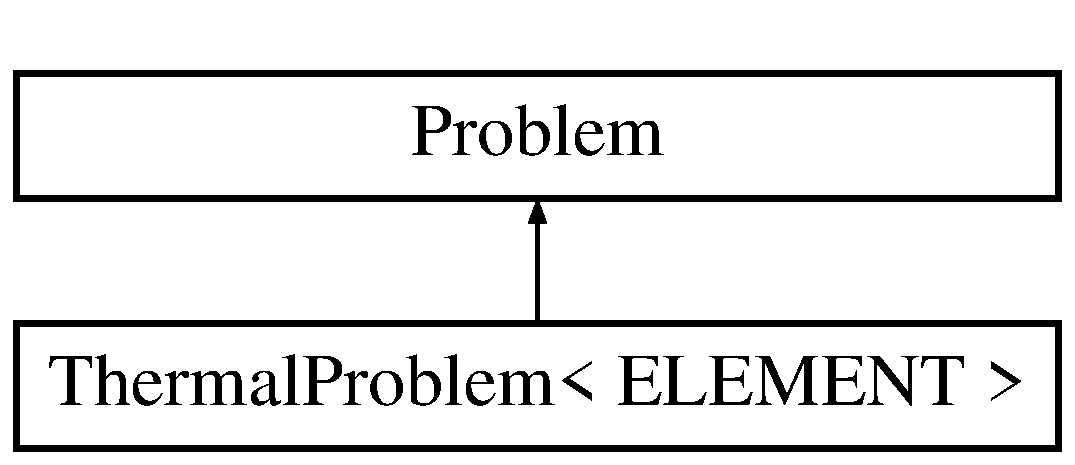
\includegraphics[height=2.000000cm]{classThermalProblem}
\end{center}
\end{figure}
\subsection*{Public Member Functions}
\begin{DoxyCompactItemize}
\item 
\hyperlink{classThermalProblem_a12ad5d383929b1ef4ed29503c5a271b0}{Thermal\+Problem} ()
\begin{DoxyCompactList}\small\item\em Constructor. \end{DoxyCompactList}\item 
\hyperlink{classThermalProblem_af563f946765bdae233c202738bf7e725}{$\sim$\+Thermal\+Problem} ()
\begin{DoxyCompactList}\small\item\em Destructor. Empty. \end{DoxyCompactList}\item 
void \hyperlink{classThermalProblem_ab2d2efaf155756144c9796b76af3ee8d}{actions\+\_\+before\+\_\+newton\+\_\+solve} ()
\begin{DoxyCompactList}\small\item\em Update the problem specs before solve (empty) \end{DoxyCompactList}\item 
void \hyperlink{classThermalProblem_ad38edfd46e049fdbc5b00bafb661f8e2}{actions\+\_\+after\+\_\+newton\+\_\+solve} ()
\begin{DoxyCompactList}\small\item\em Update the problem after solve (empty) \end{DoxyCompactList}\item 
void \hyperlink{classThermalProblem_a40bda0a4d45851f7e45dc461107d7c0f}{actions\+\_\+before\+\_\+adapt} ()
\begin{DoxyCompactList}\small\item\em Actions before adapt\+:(empty) \end{DoxyCompactList}\item 
void \hyperlink{classThermalProblem_aa085f248542811385fefe623a9193fd8}{doc\+\_\+solution} ()
\begin{DoxyCompactList}\small\item\em Doc the solution. \end{DoxyCompactList}\item 
Elastic\+Rectangular\+Quad\+Mesh$<$ E\+L\+E\+M\+E\+NT $>$ $\ast$ \hyperlink{classThermalProblem_ac1ebc681e22c65c384aa63a7e9da6129}{mesh\+\_\+pt} ()
\begin{DoxyCompactList}\small\item\em Overloaded version of the problem\textquotesingle{}s access function to the mesh. Recasts the pointer to the base Mesh object to the actual mesh type. \end{DoxyCompactList}\end{DoxyCompactItemize}
\subsection*{Private Attributes}
\begin{DoxyCompactItemize}
\item 
Doc\+Info \hyperlink{classThermalProblem_ae03e6df96a793f3735d1674e4e8a6cb3}{Doc\+\_\+info}
\begin{DoxyCompactList}\small\item\em Doc\+Info object. \end{DoxyCompactList}\end{DoxyCompactItemize}


\subsection{Detailed Description}
\subsubsection*{template$<$class E\+L\+E\+M\+E\+NT$>$\newline
class Thermal\+Problem$<$ E\+L\+E\+M\+E\+N\+T $>$}

2D Thermoelasticity problem on rectangular domain, discretised with refineable elements. The specific type of element is specified via the template parameter. 

Definition at line 254 of file thermo.\+cc.



\subsection{Constructor \& Destructor Documentation}
\mbox{\Hypertarget{classThermalProblem_a12ad5d383929b1ef4ed29503c5a271b0}\label{classThermalProblem_a12ad5d383929b1ef4ed29503c5a271b0}} 
\index{Thermal\+Problem@{Thermal\+Problem}!Thermal\+Problem@{Thermal\+Problem}}
\index{Thermal\+Problem@{Thermal\+Problem}!Thermal\+Problem@{Thermal\+Problem}}
\subsubsection{\texorpdfstring{Thermal\+Problem()}{ThermalProblem()}}
{\footnotesize\ttfamily template$<$class E\+L\+E\+M\+E\+NT $>$ \\
\hyperlink{classThermalProblem}{Thermal\+Problem}$<$ E\+L\+E\+M\+E\+NT $>$\+::\hyperlink{classThermalProblem}{Thermal\+Problem} (\begin{DoxyParamCaption}{ }\end{DoxyParamCaption})}



Constructor. 

Constructor for Convection problem. 

Definition at line 297 of file thermo.\+cc.



References Global\+\_\+\+Physical\+\_\+\+Variables\+::\+Alpha, and Global\+\_\+\+Physical\+\_\+\+Variables\+::\+Constitutive\+\_\+law\+\_\+pt.

\mbox{\Hypertarget{classThermalProblem_af563f946765bdae233c202738bf7e725}\label{classThermalProblem_af563f946765bdae233c202738bf7e725}} 
\index{Thermal\+Problem@{Thermal\+Problem}!````~Thermal\+Problem@{$\sim$\+Thermal\+Problem}}
\index{````~Thermal\+Problem@{$\sim$\+Thermal\+Problem}!Thermal\+Problem@{Thermal\+Problem}}
\subsubsection{\texorpdfstring{$\sim$\+Thermal\+Problem()}{~ThermalProblem()}}
{\footnotesize\ttfamily template$<$class E\+L\+E\+M\+E\+NT$>$ \\
\hyperlink{classThermalProblem}{Thermal\+Problem}$<$ E\+L\+E\+M\+E\+NT $>$\+::$\sim$\hyperlink{classThermalProblem}{Thermal\+Problem} (\begin{DoxyParamCaption}{ }\end{DoxyParamCaption})\hspace{0.3cm}{\ttfamily [inline]}}



Destructor. Empty. 



Definition at line 263 of file thermo.\+cc.



\subsection{Member Function Documentation}
\mbox{\Hypertarget{classThermalProblem_ad38edfd46e049fdbc5b00bafb661f8e2}\label{classThermalProblem_ad38edfd46e049fdbc5b00bafb661f8e2}} 
\index{Thermal\+Problem@{Thermal\+Problem}!actions\+\_\+after\+\_\+newton\+\_\+solve@{actions\+\_\+after\+\_\+newton\+\_\+solve}}
\index{actions\+\_\+after\+\_\+newton\+\_\+solve@{actions\+\_\+after\+\_\+newton\+\_\+solve}!Thermal\+Problem@{Thermal\+Problem}}
\subsubsection{\texorpdfstring{actions\+\_\+after\+\_\+newton\+\_\+solve()}{actions\_after\_newton\_solve()}}
{\footnotesize\ttfamily template$<$class E\+L\+E\+M\+E\+NT$>$ \\
void \hyperlink{classThermalProblem}{Thermal\+Problem}$<$ E\+L\+E\+M\+E\+NT $>$\+::actions\+\_\+after\+\_\+newton\+\_\+solve (\begin{DoxyParamCaption}{ }\end{DoxyParamCaption})\hspace{0.3cm}{\ttfamily [inline]}}



Update the problem after solve (empty) 



Definition at line 269 of file thermo.\+cc.

\mbox{\Hypertarget{classThermalProblem_a40bda0a4d45851f7e45dc461107d7c0f}\label{classThermalProblem_a40bda0a4d45851f7e45dc461107d7c0f}} 
\index{Thermal\+Problem@{Thermal\+Problem}!actions\+\_\+before\+\_\+adapt@{actions\+\_\+before\+\_\+adapt}}
\index{actions\+\_\+before\+\_\+adapt@{actions\+\_\+before\+\_\+adapt}!Thermal\+Problem@{Thermal\+Problem}}
\subsubsection{\texorpdfstring{actions\+\_\+before\+\_\+adapt()}{actions\_before\_adapt()}}
{\footnotesize\ttfamily template$<$class E\+L\+E\+M\+E\+NT$>$ \\
void \hyperlink{classThermalProblem}{Thermal\+Problem}$<$ E\+L\+E\+M\+E\+NT $>$\+::actions\+\_\+before\+\_\+adapt (\begin{DoxyParamCaption}{ }\end{DoxyParamCaption})\hspace{0.3cm}{\ttfamily [inline]}}



Actions before adapt\+:(empty) 



Definition at line 272 of file thermo.\+cc.

\mbox{\Hypertarget{classThermalProblem_ab2d2efaf155756144c9796b76af3ee8d}\label{classThermalProblem_ab2d2efaf155756144c9796b76af3ee8d}} 
\index{Thermal\+Problem@{Thermal\+Problem}!actions\+\_\+before\+\_\+newton\+\_\+solve@{actions\+\_\+before\+\_\+newton\+\_\+solve}}
\index{actions\+\_\+before\+\_\+newton\+\_\+solve@{actions\+\_\+before\+\_\+newton\+\_\+solve}!Thermal\+Problem@{Thermal\+Problem}}
\subsubsection{\texorpdfstring{actions\+\_\+before\+\_\+newton\+\_\+solve()}{actions\_before\_newton\_solve()}}
{\footnotesize\ttfamily template$<$class E\+L\+E\+M\+E\+NT$>$ \\
void \hyperlink{classThermalProblem}{Thermal\+Problem}$<$ E\+L\+E\+M\+E\+NT $>$\+::actions\+\_\+before\+\_\+newton\+\_\+solve (\begin{DoxyParamCaption}{ }\end{DoxyParamCaption})\hspace{0.3cm}{\ttfamily [inline]}}



Update the problem specs before solve (empty) 



Definition at line 266 of file thermo.\+cc.

\mbox{\Hypertarget{classThermalProblem_aa085f248542811385fefe623a9193fd8}\label{classThermalProblem_aa085f248542811385fefe623a9193fd8}} 
\index{Thermal\+Problem@{Thermal\+Problem}!doc\+\_\+solution@{doc\+\_\+solution}}
\index{doc\+\_\+solution@{doc\+\_\+solution}!Thermal\+Problem@{Thermal\+Problem}}
\subsubsection{\texorpdfstring{doc\+\_\+solution()}{doc\_solution()}}
{\footnotesize\ttfamily template$<$class E\+L\+E\+M\+E\+NT $>$ \\
void \hyperlink{classThermalProblem}{Thermal\+Problem}$<$ E\+L\+E\+M\+E\+NT $>$\+::doc\+\_\+solution (\begin{DoxyParamCaption}{ }\end{DoxyParamCaption})}



Doc the solution. 



Definition at line 386 of file thermo.\+cc.



Referenced by main().

\mbox{\Hypertarget{classThermalProblem_ac1ebc681e22c65c384aa63a7e9da6129}\label{classThermalProblem_ac1ebc681e22c65c384aa63a7e9da6129}} 
\index{Thermal\+Problem@{Thermal\+Problem}!mesh\+\_\+pt@{mesh\+\_\+pt}}
\index{mesh\+\_\+pt@{mesh\+\_\+pt}!Thermal\+Problem@{Thermal\+Problem}}
\subsubsection{\texorpdfstring{mesh\+\_\+pt()}{mesh\_pt()}}
{\footnotesize\ttfamily template$<$class E\+L\+E\+M\+E\+NT$>$ \\
Elastic\+Rectangular\+Quad\+Mesh$<$E\+L\+E\+M\+E\+NT$>$$\ast$ \hyperlink{classThermalProblem}{Thermal\+Problem}$<$ E\+L\+E\+M\+E\+NT $>$\+::mesh\+\_\+pt (\begin{DoxyParamCaption}{ }\end{DoxyParamCaption})\hspace{0.3cm}{\ttfamily [inline]}}



Overloaded version of the problem\textquotesingle{}s access function to the mesh. Recasts the pointer to the base Mesh object to the actual mesh type. 



Definition at line 280 of file thermo.\+cc.



\subsection{Member Data Documentation}
\mbox{\Hypertarget{classThermalProblem_ae03e6df96a793f3735d1674e4e8a6cb3}\label{classThermalProblem_ae03e6df96a793f3735d1674e4e8a6cb3}} 
\index{Thermal\+Problem@{Thermal\+Problem}!Doc\+\_\+info@{Doc\+\_\+info}}
\index{Doc\+\_\+info@{Doc\+\_\+info}!Thermal\+Problem@{Thermal\+Problem}}
\subsubsection{\texorpdfstring{Doc\+\_\+info}{Doc\_info}}
{\footnotesize\ttfamily template$<$class E\+L\+E\+M\+E\+NT$>$ \\
Doc\+Info \hyperlink{classThermalProblem}{Thermal\+Problem}$<$ E\+L\+E\+M\+E\+NT $>$\+::Doc\+\_\+info\hspace{0.3cm}{\ttfamily [private]}}



Doc\+Info object. 



Definition at line 289 of file thermo.\+cc.



The documentation for this class was generated from the following file\+:\begin{DoxyCompactItemize}
\item 
\hyperlink{thermo_8cc}{thermo.\+cc}\end{DoxyCompactItemize}

\chapter{File Documentation}
\hypertarget{thermo_8cc}{}\section{thermo.\+cc File Reference}
\label{thermo_8cc}\index{thermo.\+cc@{thermo.\+cc}}
\subsection*{Classes}
\begin{DoxyCompactItemize}
\item 
class \hyperlink{classQThermalPVDElement}{Q\+Thermal\+P\+V\+D\+Element$<$ D\+I\+M $>$}
\item 
class \hyperlink{classThermalProblem}{Thermal\+Problem$<$ E\+L\+E\+M\+E\+N\+T $>$}
\end{DoxyCompactItemize}
\subsection*{Namespaces}
\begin{DoxyCompactItemize}
\item 
 \hyperlink{namespaceGlobal__Physical__Variables}{Global\+\_\+\+Physical\+\_\+\+Variables}
\begin{DoxyCompactList}\small\item\em Namespace for the physical parameters in the problem. \end{DoxyCompactList}\end{DoxyCompactItemize}
\subsection*{Functions}
\begin{DoxyCompactItemize}
\item 
int \hyperlink{thermo_8cc_a3c04138a5bfe5d72780bb7e82a18e627}{main} (int argc, char $\ast$$\ast$argv)
\begin{DoxyCompactList}\small\item\em Driver code for 2D Thermoelasticity problem. \end{DoxyCompactList}\end{DoxyCompactItemize}
\subsection*{Variables}
\begin{DoxyCompactItemize}
\item 
double \hyperlink{namespaceGlobal__Physical__Variables_aa2e802ee7cc8e1ac900ba94c3ce86eb7}{Global\+\_\+\+Physical\+\_\+\+Variables\+::\+Alpha} =0.\+0
\begin{DoxyCompactList}\small\item\em Thermal expansion coefficient. \end{DoxyCompactList}\item 
double \hyperlink{namespaceGlobal__Physical__Variables_a09a019474b7405b35da2437f7779bc7e}{Global\+\_\+\+Physical\+\_\+\+Variables\+::E} = 1.\+0
\begin{DoxyCompactList}\small\item\em Young\textquotesingle{}s modulus for solid mechanics. \end{DoxyCompactList}\item 
double \hyperlink{namespaceGlobal__Physical__Variables_a3962c36313826b19f216f6bbbdd6a477}{Global\+\_\+\+Physical\+\_\+\+Variables\+::\+Nu} = 0.\+3
\begin{DoxyCompactList}\small\item\em Poisson ratio for solid mechanics. \end{DoxyCompactList}\item 
Constitutive\+Law $\ast$ \hyperlink{namespaceGlobal__Physical__Variables_a2a37fb040c832ee7a086bb13bb02a100}{Global\+\_\+\+Physical\+\_\+\+Variables\+::\+Constitutive\+\_\+law\+\_\+pt}
\begin{DoxyCompactList}\small\item\em We need a constitutive law for the solid mechanics. \end{DoxyCompactList}\end{DoxyCompactItemize}


\subsection{Function Documentation}
\mbox{\Hypertarget{thermo_8cc_a3c04138a5bfe5d72780bb7e82a18e627}\label{thermo_8cc_a3c04138a5bfe5d72780bb7e82a18e627}} 
\index{thermo.\+cc@{thermo.\+cc}!main@{main}}
\index{main@{main}!thermo.\+cc@{thermo.\+cc}}
\subsubsection{\texorpdfstring{main()}{main()}}
{\footnotesize\ttfamily int main (\begin{DoxyParamCaption}\item[{int}]{argc,  }\item[{char $\ast$$\ast$}]{argv }\end{DoxyParamCaption})}



Driver code for 2D Thermoelasticity problem. 



Definition at line 410 of file thermo.\+cc.



References Global\+\_\+\+Physical\+\_\+\+Variables\+::\+Alpha, Global\+\_\+\+Physical\+\_\+\+Variables\+::\+Constitutive\+\_\+law\+\_\+pt, Thermal\+Problem$<$ E\+L\+E\+M\+E\+N\+T $>$\+::doc\+\_\+solution(), Global\+\_\+\+Physical\+\_\+\+Variables\+::E, and Global\+\_\+\+Physical\+\_\+\+Variables\+::\+Nu.


\hypertarget{thermo_8txt__doxygenified_8h}{}\section{thermo.\+txt\+\_\+doxygenified.\+h File Reference}
\label{thermo_8txt__doxygenified_8h}\index{thermo.\+txt\+\_\+doxygenified.\+h@{thermo.\+txt\+\_\+doxygenified.\+h}}

%--- End generated contents ---

% Index
\backmatter
\newpage
\phantomsection
\clearemptydoublepage
\addcontentsline{toc}{chapter}{Index}
\printindex

